\documentclass[a4paper,12pt,french]{article}

\usepackage[]{../../../Style}

\pagestyle{empty}

\begin{document}

\newcommand{\contenua}{
\begin{centrer}
\begin{tikzpicture}
\begin{axis}[
styleglobal,
hauteurproptick,
width=0.7*\linewidth,
xmin=-7, xmax=7,
ymin=-4.5, ymax=6,
xtick distance=1,
ytick distance=1,
domain=(-7:7),
]
\addplot[styleplot]{x^2} node[pos=0.55,right] {$\mathscr C_f:\fbox{a>0}$};
\addplot[styleplot,color=red,domain=(-6:-2)]{3*(x+4)^2-4} node[pos=0.82,left] {$\mathscr C_g:\fbox{a>0}$};
\addplot[color=blue,styleplot]{2-0.25*(x-1)^2} node[pos=0.8,right] {$\mathscr C_h:\fbox{a<0}$};
\end{axis}
\end{tikzpicture}
\end{centrer}}

\newcommand{\contenub}{
\begin{center}
\begin{tikzpicture}
\begin{axis}[
styleglobal,
hauteurproptick,
width=0.7*\linewidth,
xmin=-3, xmax=5,
ymin=-1.5, ymax=1.5,
xtick distance=1,
ytick distance=1,
domain=(-6:6),
]
\addplot[styleplot]{0.7-0.5*(x-1.3)^2} node[pos=0.53,right] {$\mathscr C_f$};
\node[stylepoint,fill=red] (S) at (1.3,0.7) {};
\node (sommet) at (2.3,1.2) {Sommet};
\draw[->,>=latex,thick] (sommet.west) to[bend right=10] (S);
\draw[color=DarkRed,thick,densely dashed] (S) -- (1.3,0) node[pos=1,below] {$s$};
\draw[color=DarkRed,thick,densely dashed] (S) -- (0,0.7) node[pos=1,left] {$f(s)$};
\end{axis}
\end{tikzpicture}
\end{center}}

\newcommand{\contenuc}{
\compo
{
\begin{center}
Si $a>0$:
\begin{tikzpicture}
\tkzTabInit[lgt=1.2,espcl=2.5]{$x$ /1, $f(x)$/2}{$- \infty$, $s$, $+ \infty$}
\tkzTabVar{+/$+ \infty$, -/ $f(s)$, +/ $+\infty$}
\end{tikzpicture}
\end{center}
}
{
\begin{center}
Si $a<0$:
\begin{tikzpicture}
\tkzTabInit[lgt=1.2,espcl=2.5]{$x$ /1, $f(x)$/2}{$- \infty$, $s$, $+ \infty$}
\tkzTabVar{-/$- \infty$, +/ $f(s)$, -/ $-\infty$}
\end{tikzpicture}
\end{center}
}}

\newcommand{\contenud}{
\begin{center}
\begin{tikzpicture}
\begin{axis}[
styleglobal,
%hauteurproptick,
width=0.7*\linewidth,
xmin=-7, xmax=7,
ymin=-4, ymax=5,
xtick distance=1,
ytick distance=2,
y post scale=0.5,
domain=(-7:7),
]
\addplot[styleplot]{x^2} node[pos=0.55,right] {$\mathscr C_f:\fbox{a>0}$};
\addplot[styleplot,color=red,domain=(-2:2)]{3*(x)^2-3} node[pos=0.54,right] {$\mathscr C_g:\fbox{a>0}$};
\addplot[color=blue,styleplot]{2-0.25*(x)^2} node[pos=0.7,right] {$\mathscr C_h:\fbox{a<0}$};
\end{axis}
\end{tikzpicture}
\end{center}}

\newcommand{\contenuee}{
\begin{centrer}
\begin{tikzpicture}
\begin{axis}[
styleglobal,
hauteurproptick,
width=0.24*\linewidth,
xmin=-2.5, xmax=2.5,
ymin=-0.5, ymax=5,
xtick distance=1,
ytick distance=1,
domain=(-6:6),
]
\addplot[styleplot]{2*x^2+1} node[pos=0.525,right] {$\mathscr C_f$};
\node[stylepoint,fill=blue,label={-60:A}] at (1,3) {};
\end{axis}
\end{tikzpicture}
\end{centrer}}

\newcommand{\contenue}{\compo{\contenuee}{\contenuee}}

\newcommand{\contenuf}{
\begin{centrer}
\begin{tikzpicture}
\begin{axis}[
styleglobal,
hauteurproptick,
width=0.95*\linewidth,
xmin=-2, xmax=6,
ymin=-1, ymax=2,
xtick distance=1,
ytick distance=1,
domain=(-6:6),
]
\addplot[styleplot]{0.5*(x-1)*(x-3)} node[pos=0.52,right] {$\mathscr C_f$};
\node[stylepoint,fill=red] (S) at (2,-0.5) {};
\node (sommet) at (3,-0.7) {Sommet};
\draw[->,>=latex,thick] (sommet.west) to[bend left=10] (S);
\node[stylepoint,fill=blue] (x1) at (1,0) {};
\node[stylepoint,fill=blue] (x2) at (3,0) {};
\node (racines) at (2,1) {Racines};
\draw[->,>=latex,thick] (racines) to[bend right=10] (x1);
\draw[->,>=latex,thick] (racines) to[bend left=10] (x2);
\end{axis}
\end{tikzpicture}
\end{centrer}
}

% Début du document
%%%%%%%%%%%%%%%%%%%

%\vfill \contenua \vfill \contenua \vfill
%
%\newpage
%
%\vfill \contenub \vfill \contenub \vfill \contenub \vfill \contenub \vfill
%
%\newpage
%
%\vfill \contenuc \vfill \contenuc \vfill \contenuc \vfill \contenuc \vfill \contenuc \vfill
%
%\newpage
%
%\contenud \vfill \contenud \vfill \contenud \vfill \contenud \vfill \contenud
%
%\newpage
%
%\contenue \vfill \contenue \vfill \contenue
%
%\newpage
%
%\contenuf \vfill \contenuf \vfill \contenuf

\contenua \contenub \contenuc \contenud \contenuee \contenuf

\end{document}
